\documentclass[11pt,a4paper]{article}
\usepackage[utf8]{inputenc}\usepackage[T1]{fontenc}
\usepackage[margin=1in]{geometry}
\usepackage{amsmath,amssymb,booktabs,array,graphicx,enumitem,xcolor,parskip,titlesec}
\usepackage[hidelinks]{hyperref}
\graphicspath{{figures/}}
\definecolor{qnavy}{RGB}{20,40,75}\definecolor{qgrey}{RGB}{90,90,90}\definecolor{qred}{RGB}{150,30,30}
\titleformat{\section}{\large\bfseries\color{qnavy}}{\thesection}{0.6em}{}
\input{MACROS.tex}
\emergencystretch=2em
\begin{document}\thispagestyle{empty}
\noindent
{\large\bfseries\color{qnavy} Report R13 --- What It Takes to Onboard a New Site}\\[2pt]
{\color{qgrey}Arm B, both tracks: $k$-shot adaptation of TCGA-trained slide models to CPTAC
(WSI), and a 450k$\rightarrow$EPIC methylation transfer whose pre-declared endpoint turned out
not to be testable --- reported as exactly that.}\\[6pt]
{\color{qgrey}\rule{\textwidth}{0.4pt}}

\medskip
\noindent 11 August 2026 \quad\textbullet\quad Quantara \quad\textbullet\quad
NSCLC RWPR study, Arm B

\section*{Summary}

Both tracks simulate the same real question: \emph{a new hospital exposes its data --- what
does the pretrained model do on day one, and how many labelled cases does adaptation need?}
Both ran against sealed cohorts under one-way logged unsealing events; every number here is
extracted mechanically from the evidence bundles by \texttt{extract\_numbers.py}.

\textbf{WSI (unsealing event \#\RWsiUnsealNum, CPTAC, \RNCptacSubtype{} patients).} Subtype
needs \emph{zero} new labels: the TCGA-trained model scores AUROC \RSubZeroFull{} zero-shot on
all \RSubZeroFullN{} CPTAC patients (curve baseline \RSubFtZero), and no $k$ in the grid
improves it by more than 2\,pp --- the answer to ``how many cases must you label'' is
$k=0$. EGFR starts at \REgfrFtZero{} zero-shot and reaches \REgfrFtTwentyFive{} at
$k=25$ --- already within 2\,pp of the $k=100$ ceiling (\REgfrFtHundred) --- despite a
measured mutation-prevalence shift from \RShiftTcgaPct\% (TCGA) to \RShiftCptacPct\%
(CPTAC-LUAD). Fine-tuning $\geq$ linear probing at every $k$ on both endpoints. The OS
endpoint was \emph{dropped by a pre-registered rule}: the staged CPTAC survival columns are
empty (0 events), so no OS claim is possible and none is made.

\textbf{Methylation (unsealing event \#\RMethUnsealNum, GSE115246 anti-PD-1 EPIC,
\RMethN{} patients).} Upstream, the R10 KEAP1 model reproduces \emph{bit-exactly} (AUROC
\RReproAuroc; identical out-of-fold SHA-256). Cross-array 450k$\rightarrow$EPIC transfer is
\emph{proven} by an orthogonal positive control: sex, called from the deposit's raw signal
intensities, is recovered by the beta-value classifier at AUROC \RSexAuroc{}
(\RSexLo--\RSexHi, permutation $p=\RSexPermP$). But the pre-declared response endpoint is
\textbf{\REOneStatus}: the GEO deposit contains arrays and \emph{no outcome labels of any
kind}. We report that, correct our own corpus inventory, and publish the measured power the
cohort would have had (minimum detectable AUROC \RMdeMin--\RMdeMax{} at $n=\RMethN$) ---
rather than manufacturing a result. This is the trust framework doing precisely what it is
for.

\section{WSI track --- design}

\begin{itemize}[leftmargin=1.2em,itemsep=2pt]
\item \textbf{Pretraining.} Gated attention-MIL over Phikon-v2 features, trained on the TCGA
spine (\RPretrainSubtypeN{} patients subtype, \RPretrainEgfrN{} EGFR) --- the same feature
space and QC as R12.
\item \textbf{Exposure.} CPTAC-LUAD/LSCC. Tumor-vs-normal slide semantics were resolved from
DICOM headers \emph{before} the config was hashed: \RSlidesTumor{} tumor H\&E slides enter;
\RSlidesNormal{} adjacent-normal and \RSlidesAmbig{} ambiguous slides are excluded and logged.
Post-QC: \RNCptacSubtype{} patients. Labels were opened only after unsealing event
\#\RWsiUnsealNum{} (\RWsiUnsealUtc; config SHA-256 \texttt{\RWsiConfigShaShort}\ldots{}
recorded in the remote event log first).
\item \textbf{Grid.} $k \in \{0, 10, 25, 50, 100\}$ labelled CPTAC patients, 8 seeds,
fine-tune vs.\ linear probe, evaluated on the never-adapted remainder each seed. EGFR is
CPTAC-LUAD-only (pre-registered: LSCC has no per-patient mutation file), $n=\RNCptacEgfr$
sequenced patients; at $k=100$ the labelled pool caps at
\REgfrKeffMin--\REgfrKeffMax{} patients/seed --- recorded as $k_\text{eff}$, a deviation
adopted at split-build time, before training.
\end{itemize}

\section{The learning curves}

\begin{center}
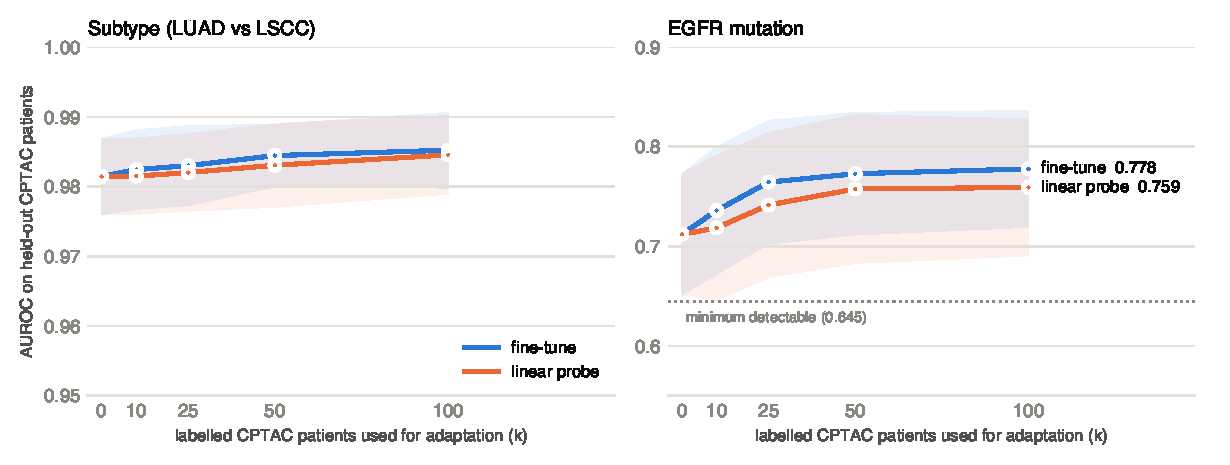
\includegraphics[width=\textwidth]{fig_learning_curves.pdf}
\end{center}
\noindent{\small\color{qgrey}8-seed mean AUROC vs.\ number of labelled CPTAC patients $k$;
bands are 95\% CIs. EGFR's measured minimum-detectable AUROC (\RWsiEgfrMde) is the dotted
line: everything the curve gains sits above what the evaluation can resolve.}

\begin{center}
\small
\input{generated_curve_table}
\end{center}
\noindent{\small\color{qgrey}Seed-mean AUROC (95\% CI). Monotone in $k$ for both methods and
endpoints (Spearman $\rho = \RSubFtSpearman$). Fine-tune $\geq$ linear probe at every point.}

The practical readings, for a site-onboarding conversation:
\begin{itemize}[leftmargin=1.2em,itemsep=2pt]
\item \textbf{Subtype: $k=0$ suffices.} Zero-shot \RSubZeroFull{} on the full cohort; the
smallest $k$ within 2\,pp of the $k=100$ ceiling is \RSubFtWithinTwoPP.
\item \textbf{EGFR: $k=25$ gets within 2\,pp of the ceiling} (\REgfrFtTwentyFive{} vs
\REgfrFtHundred). Zero-shot is \REgfrFtZero{} --- usable but visibly below ceiling, and this
under a real distribution shift: EGFR-mutant prevalence is \RShiftTcgaMut/\RShiftTcgaWt{}
(\RShiftTcgaPct\%) in TCGA training data vs \RShiftCptacMut/\RShiftCptacWt{}
(\RShiftCptacPct\%) in CPTAC-LUAD --- a \RShiftPP\,pp label shift the adaptation absorbs.
\item \textbf{Power, stated:} \input{generated_wsi_power_statement}
\item \textbf{OS: dropped, not fudged.} The pre-registered maturity rule fired before any Arm-B
training: \input{generated_os_power_statement}
\end{itemize}

\section{Methylation track --- 450k$\rightarrow$EPIC under the trust framework}

The scenario: adapt the R10 KEAP1-phenotype model (450k array, TCGA) plus an OS Cox head to a
sealed EPIC-array anti-PD-1 cohort (GSE115246, $n=\RMethN$: \RMethDiscovery{} discovery /
\RMethValidation{} validation, PMID \RMethPubmed), with anti-PD-1 response as the
pre-declared primary endpoint. Everything was frozen and hashed before the unseal
(\texttt{\RMethConfigShaShort}\ldots, event \#\RMethUnsealNum, \RMethUnsealUtc).

\textbf{Step 1 --- the starting point reproduces exactly.} Rebuilt from raw inputs, the R10
pipeline returns AUROC \RReproAuroc{} with \emph{bit-identical} out-of-fold predictions
(SHA-256 \texttt{\RReproOofSha}\ldots{} equals the R10 archive) and the sex control at
\RReproSexControl.

\textbf{Step 2 --- the array transfer is proven, not assumed.} \RRetainedOnEpicPct\% of the
\RRetainedProbes{} retained 450k probes exist on EPIC, including all \RKeapActive{} active
(non-zero-coefficient) KEAP1-model probes. Per-probe means correlate at $r=\RXArrayPearson$
across arrays with a mean absolute beta shift of \RXArrayMeanShift{} (over \RXArrayNProbes{}
probes) --- which is why the pre-declared primary transform re-centres probes within the
target cohort. The end-to-end control: sex, computed from the deposit's signal intensities
(chrX/chrY, minfi logic --- \emph{not} deposited metadata, which carries no sex field), is
recovered by the transferred beta-value classifier at \textbf{AUROC \RSexAuroc}
(\RSexLo--\RSexHi; \RSexMale{} male / \RSexFemale{} female; permutation
$p=\RSexPermP$ over \RSexNPerm{} shuffles). A deployed-model batch check finds no
cohort-membership artifact (discovery-vs-validation AUROC \RBatchAuroc, $p=\RBatchPermP$).

\textbf{Step 3 --- the endpoint is not testable, and we say so.} The deposit's only
sample-level fields are disease status (constant), tissue (constant) and cohort. \textbf{No
responder/non-responder label, no PFS, no OS, no event field was deposited} --- verified
against the series matrix and independently against the live GEO record. The response data
exist only in the paper's paywalled supplement. Verdicts, exactly as recorded:
E1 response AUROC --- \textbf{\REOneStatus}; E2 survival association --- \textbf{\RETwoStatus}
(the TCGA Cox score, internal C-index \ROsCoxCindex{} (\ROsCoxLo--\ROsCoxHi), \emph{is}
computed on all \RMethN{} samples, so the transfer itself is demonstrated).
This finding \textbf{corrects our own corpus inventory}, whose row ``GSE115246 $\mid$ 81 EPIC
anti-PD-1 responder/non-responder'' overstated the deposit: the arrays are there, the response
labels are not. One per-sample table mapping EPIMMUNE IDs to RECIST best overall response
would unblock the entire pre-registered analysis unchanged.

\textbf{Step 4 --- the power the cohort would have had.} Computed against the realized score
vector on these \RMethN{} samples, across plausible responder rates:

\begin{center}
\small
\input{generated_mde_table}
\end{center}
\noindent{\small\color{qgrey}Even with labels, only a large effect
(AUROC $\geq$ \RMdeMin--\RMdeMax) was ever detectable at $n=\RMethN$ --- the pre-declared
honest-inconclusive was the likely outcome. This mirrors R07's property, now measured on the
realized scores rather than assumed.}

\section{Why the null track matters for the study}

A system that produces analyses on new data is only trustworthy if it visibly refuses to
produce them when the data cannot support them. This arm delivered three such refusals in one
run --- the OS drop on CPTAC (empty survival columns), the response endpoint on GSE115246 (no
deposited labels), and the survival endpoint on GSE115246 (same) --- while simultaneously
proving, via positive controls, that the machinery finds real signal where it exists
(sex at \RSexAuroc{} across arrays; subtype at \RSubZeroFull{} across sites). The refusals are
credible \emph{because} the controls fire.

\section{Gates}

WSI track: all \RNGatesWsiPass{} gate-carrying checks pass; the eighth row, \texttt{g8}, is
pre-declared as reported-not-gated. Methylation track: all \RNGatesMeth{} pass.

\begin{center}
\small
\input{generated_gates_wsi}
\end{center}

\begin{center}
\small
\input{generated_gates_meth}
\end{center}

\section{Reproducing this report}

\begin{itemize}[leftmargin=1.2em,itemsep=1pt]
\item Every number: \texttt{python3 extract\_numbers.py}; figure:
\texttt{python3 make\_figures.py}. Evidence: verbatim copies of
\texttt{nsclc-rwpr-study/armB/evidence/} and \texttt{armB-meth/evidence/} (runs of
2026-08-10) under \texttt{evidence/armB-wsi/} and \texttt{evidence/armB-meth/}; the WSI
bundle additionally carries \texttt{config.yaml}, whose SHA-256 equals the
\texttt{config\_sha256} in its \texttt{results.json}.
\item Any curve point can be recomputed from the per-seed out-of-fold files, e.g.
\begin{quote}\small\begin{verbatim}
python3 -c "
import numpy as np; from sklearn.metrics import roc_auc_score
d=np.loadtxt('evidence/armB-wsi/oof_egfr_finetune_k25_seed0.csv',
             delimiter=',',skiprows=1,usecols=(2,3))
print(roc_auc_score(d[:,0].astype(int), d[:,1]))"
\end{verbatim}\end{quote}
\item The independent audit (\texttt{evidence/armB-meth/audit\_armb\_meth.json}) recomputes
the R10 reproduction, probe overlap, sex transfer and the full MDE grid; all match the run.
\item Unsealing events: \texttt{evidence/armB-meth/unsealing\_events\_snapshot.jsonl};
the remote append-only log lives in the study bucket under
\texttt{nsclc-rwpr-study/}\allowbreak\texttt{\_provenance/}.
\end{itemize}

\end{document}
